In order to reduce the necessary costs to design this constellation, some other configurations have been discussed. The Walker Delta Configuration (WDC) represents the most general constellation for a given inclination different to 90 degrees, i.e. 75 degrees. The WDC is a uniform based 360 degrees generated configuration with equidistant orbits, which implies a certain redundant Earth coverage. However, this can be solved by generating a 180 degrees constellation - Semi Walker Delta Configuration (SWDC) - which can also fulfil global coverage although having some disadvantages. One of these drawbacks is the fact that a gap is obtained, as it is discussed in \cite[Chapter 3, Section 4]{annex1}.

To avoid the gap, adding planes to the SWDC can be contemplated. In result, different configurations distributed around the Earth can be described and set in order to fulfil global coverage. As discussed before, the SWDC constellation is generated around 180 degrees whereas the Walker Delta Constellation is a 360 degrees generated configuration. This Mixed Walker Delta (MWDC) is the result of adding some planes to the SWDC, thus a constellation can be generated for different degree values, such as 200, 225, 240, etc. 

\begin{figure}[h]
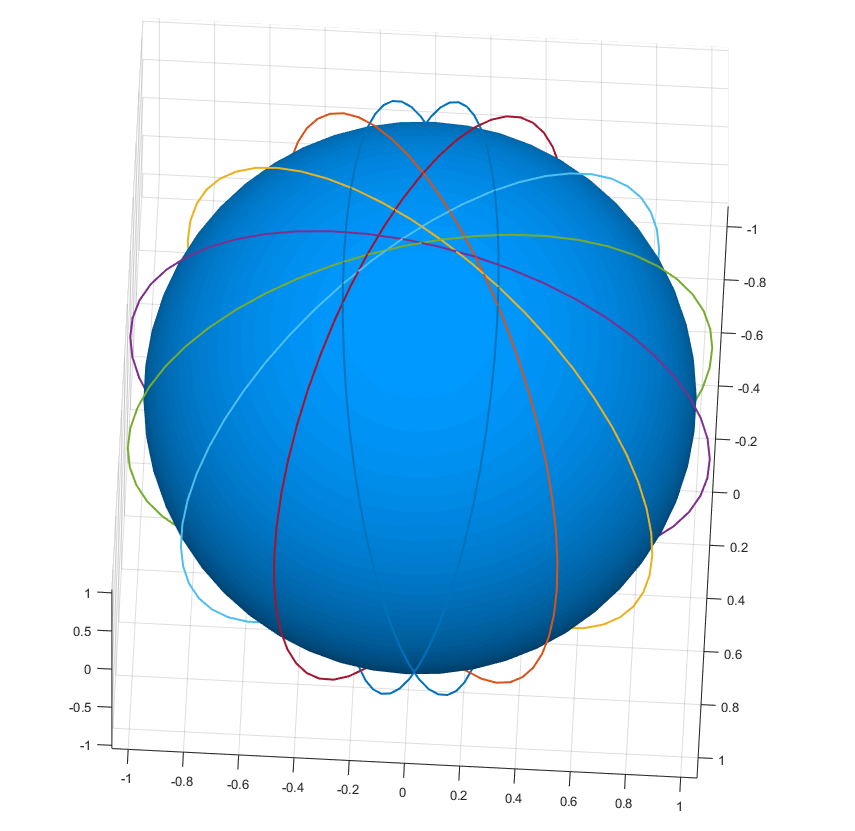
\includegraphics[width=8cm]{MWDC}
\centering
\caption{8 plane based MWDC generated for 210 degrees}
\end{figure}